\textcolor{blue}{Problem 1}

5.12 Shannon codes and Huffman codes.\quad Consider a random variable $X$ that takes on four values with probabilities $\left(\dfrac{1}{3},\dfrac{1}{3},\dfrac{1}{4},\dfrac{1}{12}\right)$.

(a) Construct a Huffman code for this random variable.

(b) Show that there exist two different sets of optimal lengths for the codewords; namely, show that codeword length assignments (1,2,3,3) and (2,2,2,2) are both optimal.

(c) Conclude that there are optimal codes with codeword lengths for some symbols that exceed the Shannon code length $\left\lceil\log\frac{1}{p(x)}\right\rceil$.

\textcolor{blue}{Solution}

(a) The Huffman tree and each variable's code are shown below.
\begin{figure}[htbp]
    \centering
	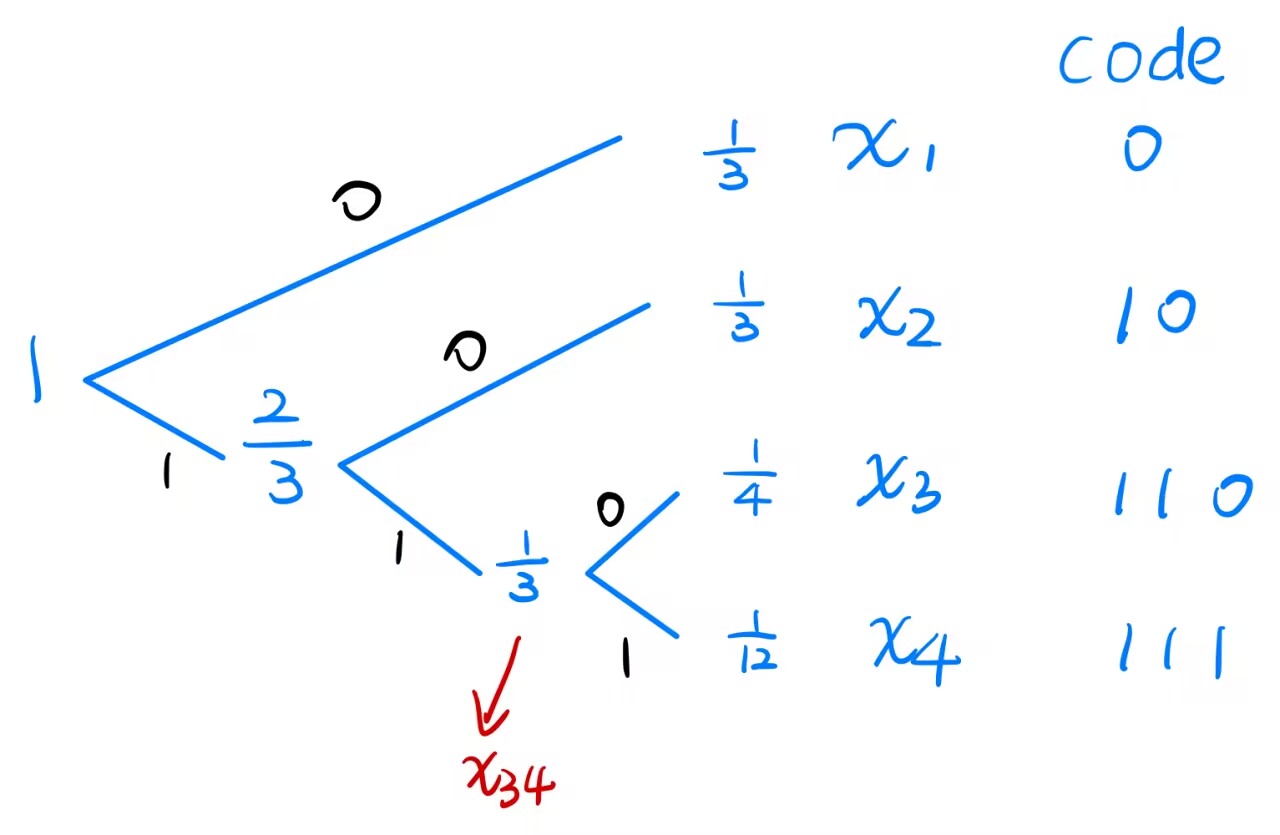
\includegraphics[width=0.5\textwidth]{../huffman1.png}
    \caption{Huffman tree 1}
    \label{fig:huffman1}
\end{figure}

(b) After merging $x_3,x_4$ and generate $x_{34}$, the probabilities of $x_1,x_2,x_{34}$ are all $\dfrac{1}{3}$. Thus, we could merge any of one node in $\left\{x_1,x_2\right\}$ with $x_{34}$ first as Figure \ref{fig:huffman1}, the length of the codes in that tree are $\left(1,2,3,3\right)$; or we can merge $x_1,x_2$ first, then merge $x_{12}$ with $x_{34}$ as Figure \ref{fig:huffman2}, the length of the codes in this tree are $\left(2,2,2,2\right)$. Both of these trees are valid Huffman trees, so these codewords are both optimal.

\begin{figure}[htbp]
    \centering
	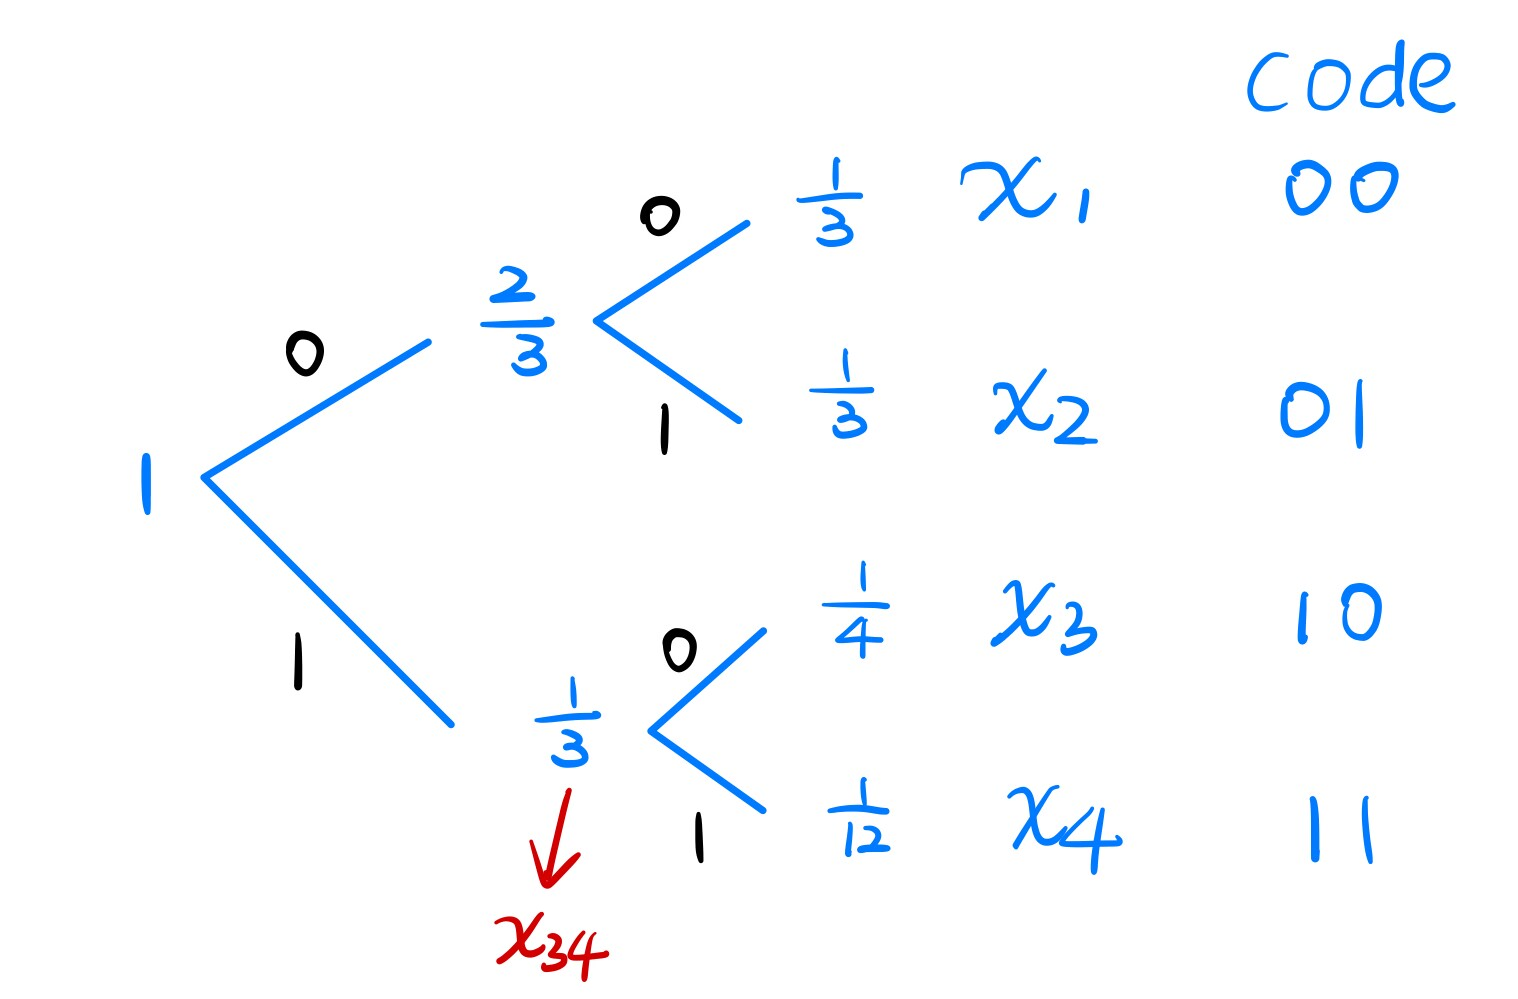
\includegraphics[width=0.5\textwidth]{../huffman2.png}
    \caption{Huffman tree 2}
    \label{fig:huffman2}
\end{figure}

And we can compute the average length of the codewords in these two trees, suppose the average length of the codewords in the first tree is $\overline{L}_1$, and the average length of the codewords in the second tree is $\overline{L}_2$, then we have

\begin{align*}
\overline{L}_1 &= \dfrac{1}{3}\times1+\dfrac{1}{3}\times2+\dfrac{1}{4}\times3+\dfrac{1}{12}\times3=2 \text{\ bits} \\
\overline{L}_2 &= \dfrac{1}{3}\times2+\dfrac{1}{3}\times2+\dfrac{1}{4}\times2+\dfrac{1}{12}\times2=2 \text{\ bits}
\end{align*}

And $\overline{L}_1=\overline{L}_2$, which also shows that the codes are both optimal.

(c) For the second way to construct the Huffman tree in Figure \ref{fig:huffman1}, we could see that $l(x_3)=3\text{\ bits}$, but according to the Shannon's code, $\left\lceil\log\frac{1}{p(x_3)}\right\rceil=\left\lceil\log4\right\rceil=2\text{\ bits}$. And Huffman code is optimal, so we have for $x_3$, $l(x_3)>\left\lceil\log\frac{1}{p(x_3)}\right\rceil$ exceeds the Shannon code length.

\newpage